\subsect{Sprint 3}{sprint3}

\underline{Fecha de inicio}: 11/08/2022

\underline{Fecha de fin}: 11/09/2022

\underline{Objetivos}:
\begin{itemize}
	\item Envío de mensajes de conexión y desconexión de usuarios.
	\item Recuperación y guardado del historial de mensajes.
	\item Soporte de conexión \enquote*{idle}.
\end{itemize}

\underline{Descripción}:
En este sprint se pretende añadir la funcionalidad de envío de mensajes de conexión y desconexión de usuarios, de
forma que se pueda notificar a los usuarios cuando ocurra cualquiera de esos eventos.\ Además, cuando el
\boldFont{primer usuario} se conecte, se recuperará el historial de mensajes del chat al que se ha conectado.\ De
manera contraria, cuando el \boldFont{último usuario} se desconecte, se guardará el historial de mensajes del chat en
el servicio de almacenamiento en la nube S3 de Amazon Web Services.\ Por último, se añadirá soporte de conexión
\enquote*{idle}, de forma que si un usuario se ausenta durante un tiempo y no realiza ninguna acción, se garantiza
que no se le desconecte del chat.

\underline{Imprevistos}:
Heroku ha eliminado su plan gratuito de despliegue de aplicaciones, por lo que se ha tenido que buscar una
alternativa para desplegar la aplicación y se ha optado por utilizar Vercel.

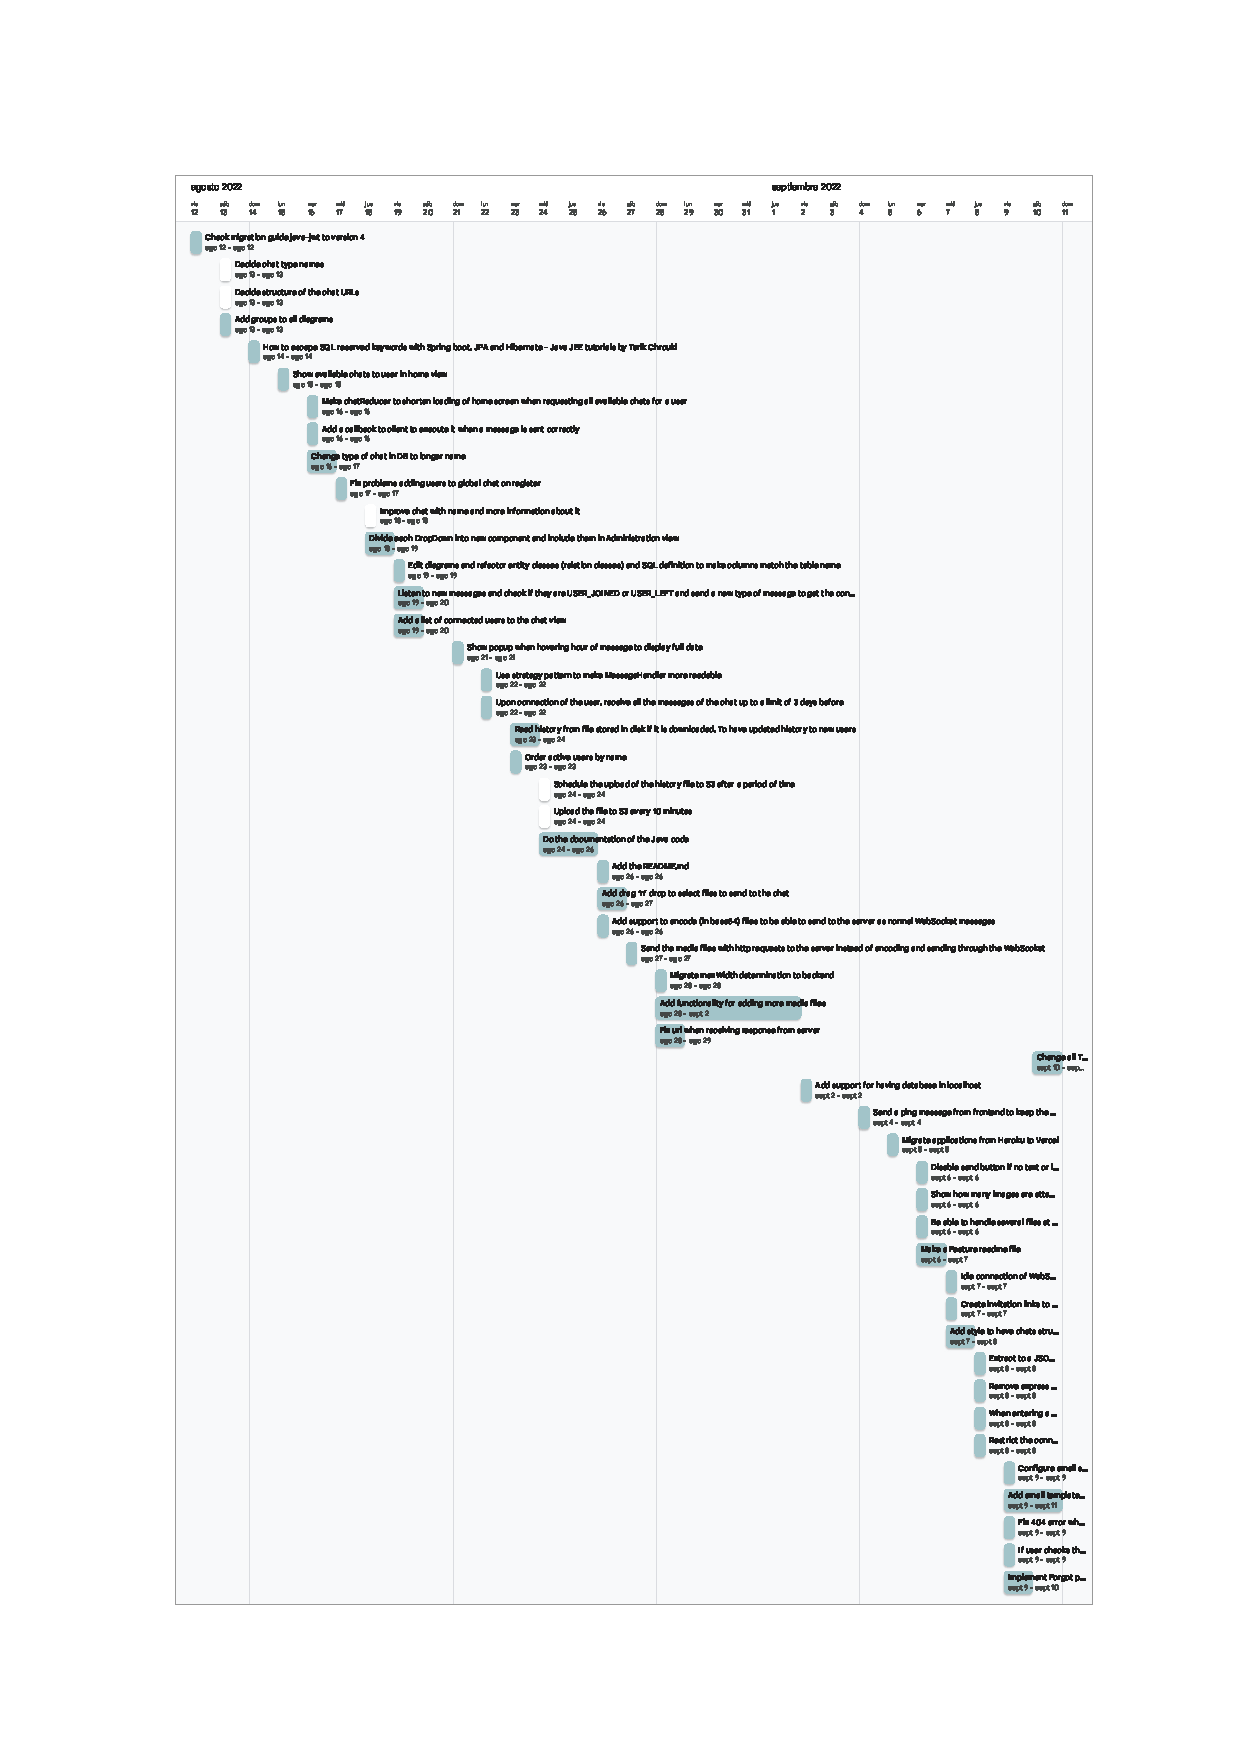
\includepdf[pages=-]{backlog/sprints/Sprint3.pdf}
